\section{ReMap System Design and Implementation}
ReMap (\autoref{fig:remap_interface}) extends the RePlay contextual search system (Chapter \ref{chapter:replay}) . RePlay enables users to search for learning videos in context while working in software, and it highlights relevant moments in video results based on the user's context and query. While RePlay helps people find results faster, the attentional cost of switching to RePlay discouraged its being used as often as it could. ReMap lowers the switching cost and load by introducing three main improvements over RePlay: searching for help using speech, making deictic references in a search query, and navigating video results using speech commands.

\subsection{Searching for Help using Speech}
ReMap uses the Web Speech \textsc{api} to detect speech by opening a browser page in the background when launched. This page can be minimized or hidden by the user. The first time it opens it asks the user to grant access to the microphone; all subsequent uses will grant access automatically. The page's JavaScript invokes continuous listening and sends the current phrase to ReMap's custom web server whenever a new word is detected.
The Web Speech \textsc{api} automatically determines when the user starts and finishes speaking, returning each phrase separately. If a phrase begins with the word \textit{``search''}, ReMap initiates a search (\autoref{fig:remap_interface}a), using the rest of the phrase as the query. Otherwise, it checks if the phrase matches any video navigation commands. If it does not, ReMap ignores it.

\subsection{Making Deictic References in a Search Query}
Especially with new software, people are often unfamiliar with an application's vocabulary but can point at application elements that are relevant to their goal. 
To alleviate the challenge of remembering app-specific terms, ReMap allows users to deictically reference interface elements and objects while speaking their query. If the user says \textit{``this''} or \textit{``that''} while clicking on a detectable element, ReMap replaces the pronoun with the reference element's name (\autoref{fig:remap_interface}b-c). Like RePlay, ReMap uses the MacOS Accessibility \textsc{api} to resolve element names. 
%This \textsc{api} can get the name and description of any element with accessibility labels \cite{Fraser2019}. Many modern applications have labeled menus, buttons, and other interface elements. Some also label canvas elements (such as text boxes, images, and graphics) though many do not. The examples in this demo use Canva (\url{canva.com}) as the primary software. Canva labels most canvas elements and interface buttons.

While ReMap is detecting a speech query, it stores a list of every detectable element clicked. Once the user is finished speaking and ReMap has obtained the final query from the server, it replaces all occurrences of \textit{``this''} and \textit{``that''} with the element names in the order they were clicked before issuing the search query.

\subsection{Navigating Video Results Using Speech Commands}
The user can speak commands to navigate video results, inspired by Chang \textit{et al.}'s recommendations \cite{Chang2019}. ReMap currently supports the following commands: \textit{``play''} (plays the first or most-recently played video), \textit{``play \{next, previous, last\}''} (plays the next/previous/last video in the list), \textit{``play \{first, second, third, fourth, fifth\} video''}, \textit{``\{next, previous, repeat\} marker''} (skips to the next or previous timeline marker, or re-starts from the current marker), and \textit{``pause''} / \textit{``stop''} (pauses the currently playing video).


\subsection{Implementation}
ReMap is implemented as a MacOS Swift application (\autoref{fig:remap_system}a). It uses socket.io to communicate between the web server and the three client interfaces (the ReMap desktop application, web speech page, and video players). The web server (\autoref{fig:remap_system}b) is implemented in Node.js. The speech engine (\autoref{fig:remap_system}c) uses the Web Speech \textsc{api}, and the video player (\autoref{fig:remap_system}d) uses the YouTube Player \textsc{api} to load and control videos. ReMap generates a unique anonymous user ID for each computer it runs on. When it opens the speech engine and video player webpages, it includes this user ID as a parameter. For video player pages, it also includes that video's index in the result list. The server keeps track of these values for each client page that opens a socket connection, so that it can pass commands it receives to the appropriate client.

\begin{figure}[t!]
\centering
  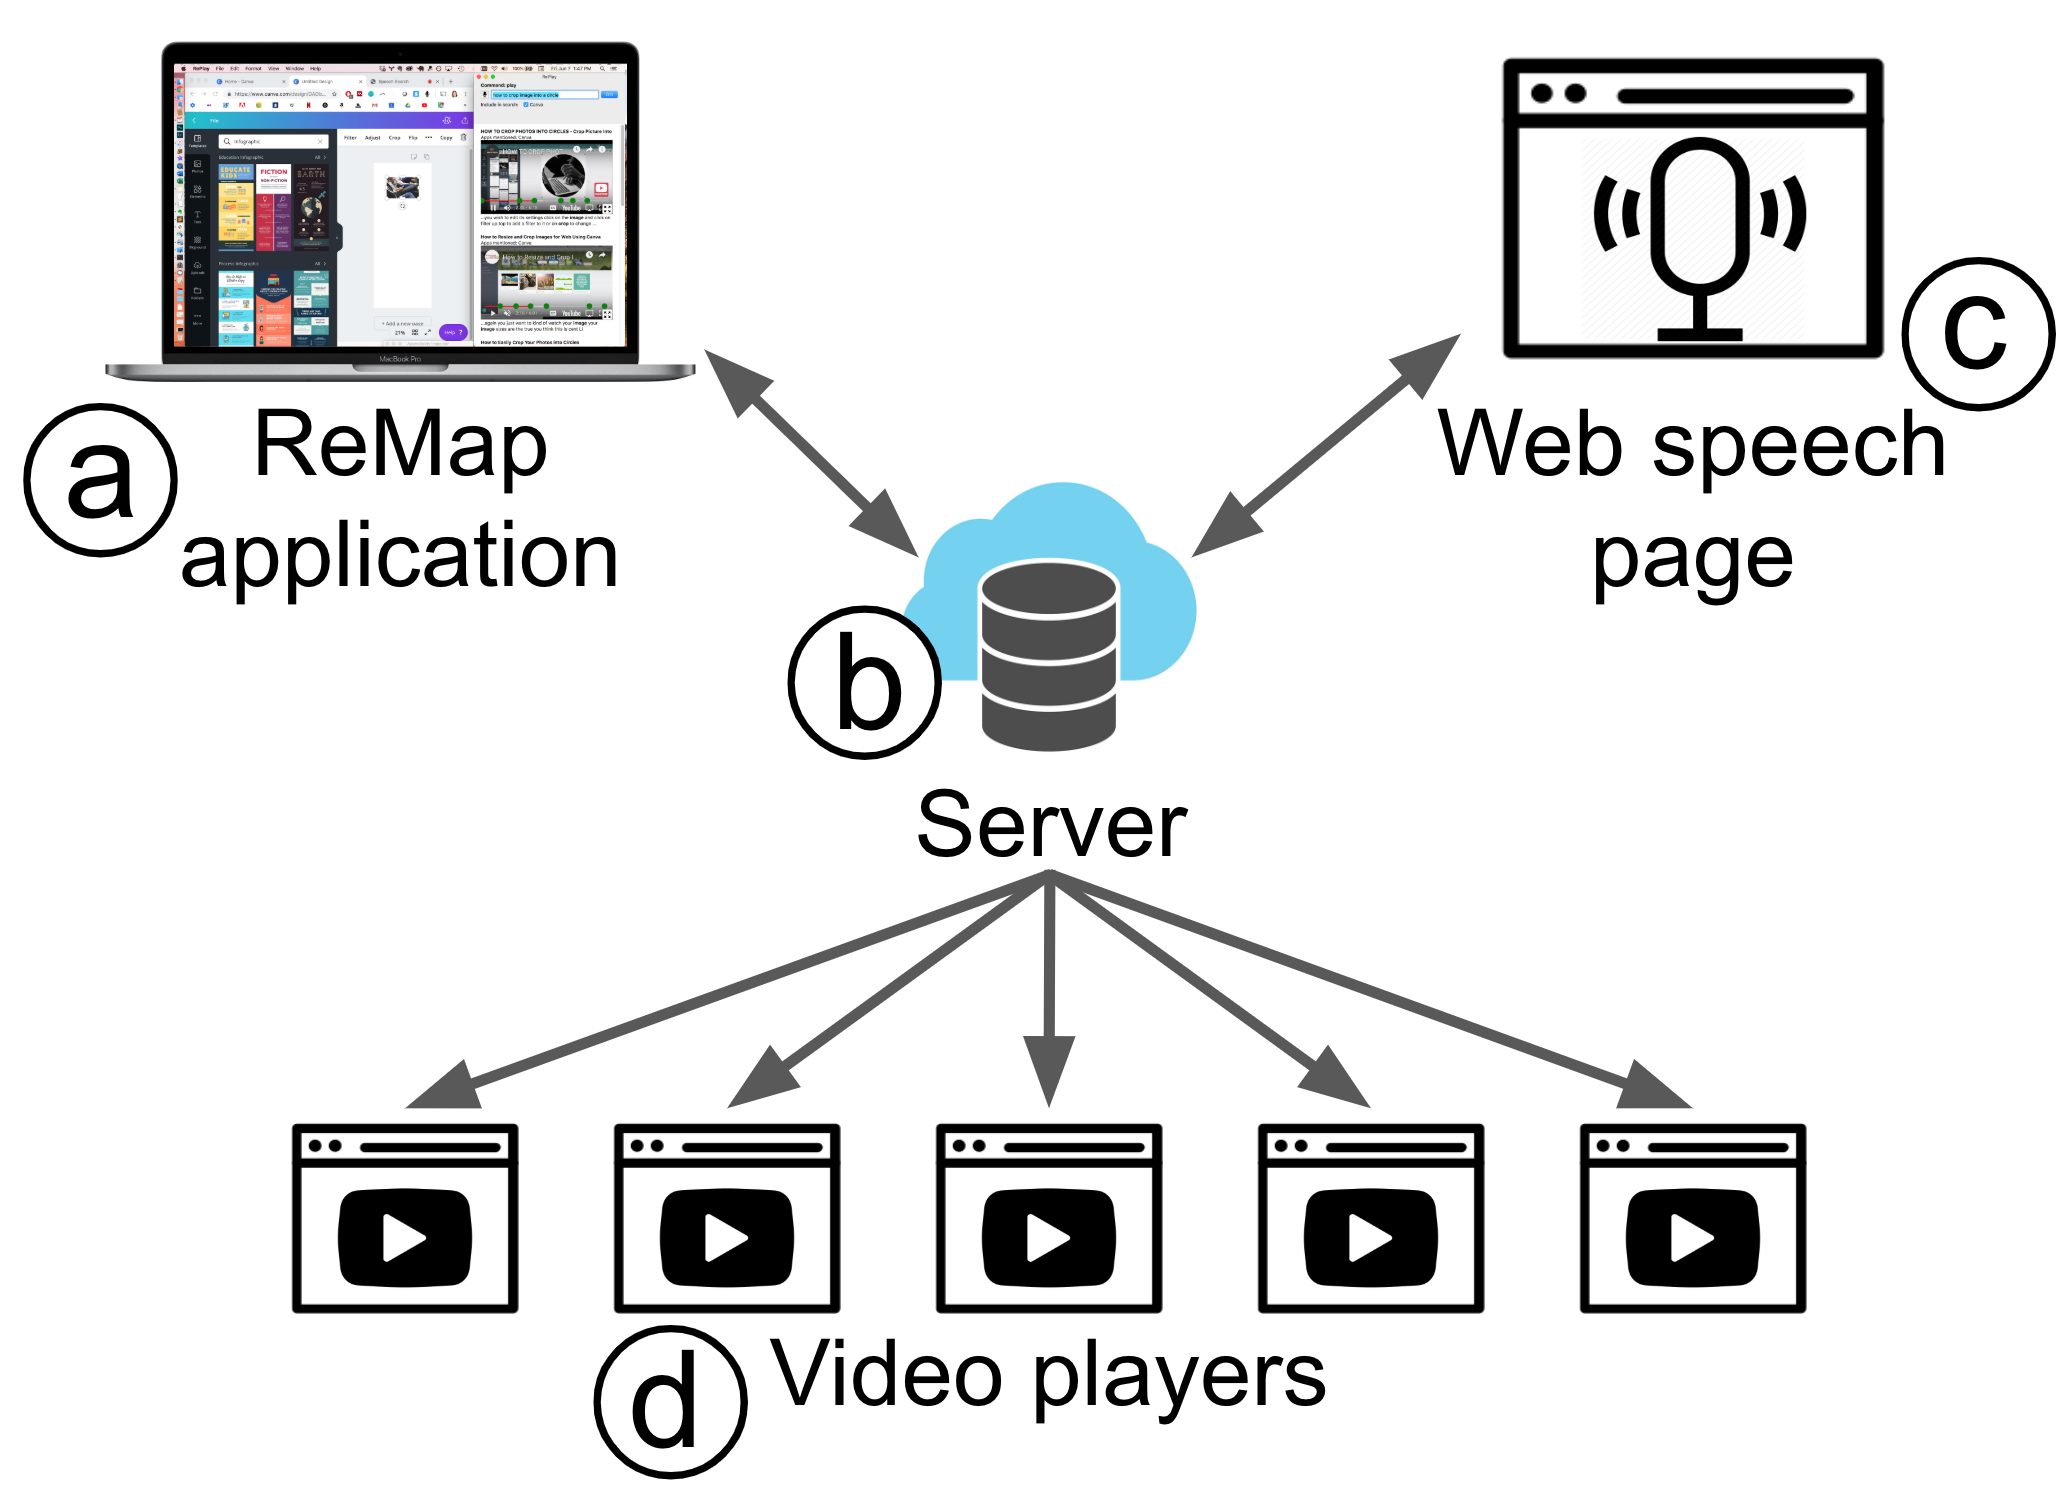
\includegraphics[width=.7\textwidth]{remap/figures/system.png}
  \caption{The ReMap system architecture. a) ReMap is a MacOS application that uses the Accessibility \textsc{api} to detect user context. b) ReMap connects to a web server, which opens c) a webpage for speech recognition, and d) a video player webpage for each result to embed in ReMap.}~\label{fig:remap_system}
\end{figure}

The web speech page determines whether a spoken phrase starts with the word \textit{``search''} and if so, sends the rest of the phrase to the server which sends it to the ReMap app as a query. If a phrase matches a video navigation command, the server sends this command to the ReMap app which then determines which video index it applies to, and returns a message to the server telling it which video player to send the command to. If the command was to play a different video than the currently playing video, ReMap also asks the server to pause the currently playing video.
